\chapter{What is a Group?}
A group is one of the most basic structures in higher mathematics.
In this chapter I will tell you only the bare minimum:
what a group is, and when two groups are the same.

\section{Definition and Examples of Groups}
\prototype{The additive group of integers $\ZZ_+$ and the cyclic group $\ZZ_m$. Just don't let yourself forget that most groups are non-commutative.}

A group consists of two pieces of data: a set $G$, and an associative binary operation $\star$ with some properties.
Before I write down the definition of a group, let me give two examples.

\begin{example}[Additive Integers]
	The pair $(\ZZ, +)$ is a group:
	$\ZZ = \left\{ \dots,-2,-1,0,1,2,\dots \right\}$ is the set
	and the associative operation is \emph{addition}.
	This operation has the following nice properties:
	\begin{itemize}
		\ii The element $0 \in \ZZ$ is an \emph{identity}:
		$a+0=0+a = a$ for any $a$.
		\ii Every element $a \in \ZZ$ has an additive \emph{inverse}: $a + (-a) = (-a) + a = 0$.
	\end{itemize}
	We call this group $\ZZ_+$.
\end{example}
\begin{abuse}
	For this chapter and the third chapter,
	I'll use $\ZZ_+$ to be clear that I'm referring to the additive group.
	However, after this part I'll start just writing $\ZZ$ like everyone else.
\end{abuse}
\begin{example}[Nonzero Rationals]
	Let $\QQ^\times$ be the set of \emph{nonzero rational numbers}.
	The pair $(\QQ^\times, \cdot)$ is a group:
	the set is $\QQ^\times$
	and the associative operation is \emph{multiplication}.

	Again we see the same two nice properties.
	\begin{itemize}
		\ii The element $1 \in \QQ^\times$ is an \emph{identity}:
		for any rational number, $a \cdot 1 = 1 \cdot a = a$.
		\ii For any rational number $x \in \QQ^\times$,
		we have an inverse $\frac{1}{x}$, such that
		\[ x \cdot \frac 1x = \frac 1x \cdot x = 1. \]
	\end{itemize}
\end{example}

From this I bet you can already guess what the definition of a group is.
\begin{definition}
	A \vocab{group} is a pair $G = (G, \star)$
	consisting of a set of elements $G$, and an associative
	binary operation $\star$ on $G$, with the following properties.
	\begin{itemize}
		\ii $G$ has an \vocab{identity element}, usually denoted $1_G$
		or just $1$, with the property that
		\[ 1_G \star g = g \star 1_G = g \text{ for all $g \in G$}. \]
		\ii Each element $g \in G$ has an \vocab{inverse}, that is, an element $h \in G$ such that \[ g \star h = h \star g = 1_G. \]
	\end{itemize}
	\label{def:group}
\end{definition}

\begin{figure}[ht]
	\centering
	\includegraphics[height=8cm]{/home/evan/Pictures/TopologicalGG/are-you-my-identity.jpg}
	\caption{The identity of a group is generally written ``$1$''.}
\end{figure}

Now that I've made clear what the criteria of a group are, let us write down some non-examples of groups.

\begin{example}[Non-Examples of Groups]
	\listhack
	\begin{itemize}
		\ii The pair $(\QQ, \cdot)$ is NOT a group.
		While there is an identity element, the element $0 \in \QQ$
		does not have an inverse.
		\ii The pair $(\ZZ, \cdot)$ is also NOT a group. (Why?)
		\ii Let $\Mat_{2 \times 2}$ be the set of $2 \times 2$ matrices.
		Then $(\Mat_{2 \times 2}, \cdot)$ (where $\times$ is matrix multiplication) is NOT a group. Indeed, even though we have an identity matrix
		\[ \left(
			\begin{array}{cc}
				1 & 0 \\ 0 & 1
			\end{array}
			\right)
		\]
		we still run into the same issue as before:
		the zero matrix does not have a multiplicative inverse.
		\ii Even if we delete the zero matrix from the set,
		the resulting structure is still not a group:
		those of you that know even a little linear algebra
		might recall that any matrix with determinant zero
		cannot have an inverse.
	\end{itemize}
\end{example}

Let's resume writing down examples of groups.

\begin{example}
	[General Linear Group]
	Let $n$ be a positive integer.
	Then $\GL_n(\RR)$ is defined as the set of $n \times n$ real matrices which have nonzero determinant.
	It turns out that with this condition, every matrix does indeed have an inverse, so $(\GL_n(\RR), \times)$ is a group, called the
	\vocab{general linear group}.
	(The fact that $\GL_n(\RR)$ is closed under $\times$ follows from the linear algebra fact that $\det (AB) = \det A \det B$.)
\end{example}
\begin{example}
	[Special Linear Group]
	Following the example above, let $\SL_n(\RR)$ denote 
	the set of $n \times n$ matrices whose determinant is actually $1$.
	Again, for linear algebra reasons
	it turns out that $(\SL_n(\RR), \times)$ is also a group, called the \vocab{special linear group}.
\end{example}

\begin{example}
	[Complex Unit Circle]
	Let $S^1$ denote the set of complex numbers $z$ with absolute value one; that is
	\[ S^1 \defeq \left\{ z \in \CC \mid \left\lvert z \right\rvert = 1 \right\}. \]
	Then $(S^1, \times)$ is a group because
	\begin{itemize}
		\ii The complex number $1 \in S^1$ serves as the identity, and
		\ii Each complex number $z \in S^1$ has an inverse $\frac 1z$ which is also in $S^1$, since $\left\lvert z\inv \right\rvert = \left\lvert z \right\rvert\inv = 1$.
	\end{itemize}
	There is one thing I ought to also check: that $z_1 \times z_2$ is actually still in $S^1$.
	But this follows from the fact that $\left\lvert z_1z_2 \right\rvert = \left\lvert z_1 \right\rvert \left\lvert z_2 \right\rvert = 1$.
\end{example}

\begin{example}
	[Addition mod $n$]
	Here is an example from number theory:
	Let $n > 1$ be an integer,
	and consider the residues modulo $n$.
	These form a group under addition.
	We call this the \vocab{cyclic group of order $n$},
	and abbreviate it as $\Zc n$, with elements $\ol 0, \ol 1, \dots$.
	\label{def:cyclic_group}
\end{example}
\begin{example}
	[Multiplication mod $p$]
	Let $p$ be a prime.
	Consider the \emph{nonzero residues modulo $p$},
	which we denote by $\Zm p$
	Then $\left( \Zm p, \times \right)$ is a group.
	\label{def:mult_mod_p}
\end{example}
\begin{ques}
	Why do we need the fact that $p$ is prime?
\end{ques}

The next two examples are fairly important ones:

\begin{example}
	[Symmetric Groups]
	Let $S_n$ be the set of permutations of $\left\{ 1,\dots,n \right\}$.
	By viewing these permutations as functions from $\left\{ 1,\dots,n \right\}$ to itself, we can consider \emph{compositions} of permutations.
	Then the pair $(S_n, \circ)$ (here $\circ$ is function composition)
	is also a group, because
	\begin{itemize}
		\ii There is an identity permutation, and
		\ii Each permutation has an inverse.
	\end{itemize}
	The group $S_n$ is called the \vocab{symmetric group} on $n$ elements.
\end{example}

\begin{example}
	[Dihedral Group]
	The \vocab{dihedral group of order $2n$}, denoted $D_{2n}$,
	is the group of symmetries of a regular $n$-gon $A_1A_2 \dots A_n$,
	which includes rotations and reflections.
	It consists of the following $2n$ elements:
	\[ \left\{ 1, r, r^2, \dots, r^{n-1}, s, sr, sr^2, \dots, sr^{n-1} \right\}. \]
	The element $r$ corresponds to rotating the $n$-gon by $\frac{2\pi}{n}$,
	while $s$ corresponds to reflecting it across the line $OA_1$
	(here $O$ is the center of the polygon).
	So $rs$ mean ``reflect then rotate'' (like with function composition,
	we read from right to left).

	In particular, $r^n = s^2 = 1$. You can also see that $r^ks = sr^{-k}$.
\end{example}

Trivia: the dihedral group $D_{12}$ is my favorite example of a non-abelian group,
and is the first group I try for any exam question of the form ``find an example\dots''.
Here is a picture of some elements of $D_{10}$.
\begin{center}
	\begin{asy}
		size(12cm);
		picture aoeu(string a, string b, string c, string d, string e,
					string x) {
			draw(dir(0)--dir(72)--dir(144)--dir(216)--dir(288)--cycle);
			MP(a, dir(0), dir(0));
			MP(b, dir(72), dir(72));
			MP(c, dir(144), dir(144));
			MP(d, dir(216), dir(216));
			MP(e, dir(288), dir(288));
			MP(x, origin, origin);
			return CC();
		}
		picture one = aoeu("1", "2", "3", "4", "5", "1");
		picture r = aoeu("5", "1", "2", "3", "4", "r");
		picture s = aoeu("1", "5", "4", "3", "2", "s");
		picture sr = aoeu("5", "4", "3", "2", "1", "sr");
		picture rs = aoeu("2", "1", "5", "4", "3", "rs");
		add(shift( (0,0) ) * one);
		add(shift( (3,0) ) * r);
		add(shift( (6,0) ) * s);
		add(shift( (9,0) ) * sr);
		add(shift( (12,0) ) * rs);
	\end{asy}
\end{center}


Note that the last two groups all share a non-property: the group operation is not in general commutative!
We leave these as a warning for the reader.
\begin{definition}
We say that a group is \vocab{abelian} if the operation is commutative and \vocab{non-abelian} otherwise.
\end{definition}

\begin{example}
	[Products of Groups]
	Let $(G, \star)$ and $(H, \ast)$ be groups.
	We can define a \vocab{product group} $(G \times H, {\cdot})$, as follows.
	The elements of the group will be ordered pairs $(g,h) \in G \times H$.
	Then
	\[ (g_1, h_1) \cdot (g_2, h_2) = (g_1 \star g_2, h_1 \ast h_2) \in G \times H
		\]
	is the group operation.
	\label{def:product_group}
\end{example}
\begin{ques}
	What are the identity and inverses of the product group?
\end{ques}

\begin{example}
	[Trivial Group]
	The \vocab{trivial group}, often denoted $0$ or $1$,
	is the group with only an identity element.
	I will use the notation $\{1\}$.
\end{example}

\begin{exercise}
	Which of these are groups?
	\begin{enumerate}[(a)]
		\ii Rational numbers with odd denominators (in simplest form), where the operation is addition.
		(This includes integers, written as $n/1$, and $0 = 0/1$).
		\ii The set of rational numbers with denominator at most $2$, where the operation is addition.
		\ii The set of rational numbers with denominator at most $2$, where the operation is multiplication.
		\ii The set of nonnegative integers, where the operation is addition.
	\end{enumerate}
\end{exercise}


\section{Properties of Groups}
\prototype{$\Zm p$ is possibly best.}
\begin{abuse}
	From now on, we'll often refer to a group $(G, \star)$ by just $G$.
	Moreover, we'll abbreviate $a \star b$ to just $ab$.
	Also, because the operation $\star$ is associative,
	we will omit unnecessary parentheses: $(ab)c = a(bc) = abc$.
\end{abuse}
\begin{abuse}
	From now on, for any $g \in G$ and $n \in \NN$ we abbreviate
	\[ g^n
		=
		\underbrace{g \star \dots \star g}_{\text{$n$ times}}.\]
	Moreover, we let $g\inv$ denote the inverse of $g$,
	and $g^{-n} = (g\inv)^n$.
\end{abuse}

If you did functional equations at the IMO, you might know that you can actually determine a lot about a function just by knowing a few properties of it.
For example, if you know that $f : \QQ \to \RR$ satisfies $f(x+y) = f(x) + f(y)$, then you actually can show that $f(x) = cx$ for some $c \in \RR$.
(This is called Cauchy's functional equation.)

In the same vein, we can try to deduce some properties that a group must have just from \Cref{def:group}.
(In fact, this really is a functional equation: $\star$ is just a function $G \times G \to G$.)

It is a law in Guam and 37 other states that I now state the following proposition.
\begin{fact}
	Let $G$ be a group.
	\begin{enumerate}[(a)]
		\ii The identity of a group is unique.
		\ii The inverse of any element is unique.
		\ii For any $g \in G$, $(g\inv)\inv = g$.
	\end{enumerate}
\end{fact}
\begin{proof}
	This is mostly just some formal ``functional-equation'' style manipulations,
	and you needn't feel bad skipping it on a first read.
	\begin{enumerate}[(a)]
		\ii If $1$ and $1'$ are identities, then $1 = 1 \star 1' = 1'$.
		\ii If $h$ and $h'$ are inverses to $g$, then $1_G = g \star h
		\implies h' = (h' \star g) \star h = 1_G \star h = h$.
		\ii Trivial; omitted. \qedhere
	\end{enumerate}
\end{proof}

Now we state a slightly more useful proposition.
\begin{proposition}
	Let $G$ be a group, and $a,b \in G$.
	Then $(ab)\inv = b\inv a\inv$.
\end{proposition}
\begin{proof}
	Direct computation. We have
	\[ (ab)(b\inv a\inv)
		= a (bb\inv) a\inv = aa\inv = 1_G. \]
	Hence $(ab)\inv = b\inv a\inv$.
	Similarly, $(b\inv a\inv)(ab) = 1_G$ as well.
\end{proof}

Finally, we state a very important lemma about groups,
which highlights why having an inverse is so valuable.
\begin{lemma}
	Let $G$ be a group, and pick a $g \in G$. 
	Then the map $G \to G$ given by
	$x \mapsto gx$
	is a bijection.
	\label{lem:group_mult_biject}
\end{lemma}
\begin{exercise}
	Check this. (Show injectivity and surjectivity directly.)
\end{exercise}
\begin{example}
	Let $G = \Zm 7$ (as in \Cref{def:mult_mod_p}) and pick $g=3$.
	The above lemma states that the map $x \mapsto 3 \cdot x$ is a bijection, and we can see this explicitly:
	\begin{align*}
		1 &\overset{\times 3}{\longmapsto} 3 \pmod 7 \\
		2 &\overset{\times 3}{\longmapsto} 6 \pmod 7 \\
		3 &\overset{\times 3}{\longmapsto} 2 \pmod 7 \\
		4 &\overset{\times 3}{\longmapsto} 5 \pmod 7 \\
		5 &\overset{\times 3}{\longmapsto} 1 \pmod 7 \\
		6 &\overset{\times 3}{\longmapsto} 4 \pmod 7.
	\end{align*}
\end{example}


The fact that the map is injective is often called the \vocab{cancellation law}.
(Why do you think so?)

\section{Isomorphisms}
\prototype{$\ZZ_+ \cong 10\ZZ_+$.}
First, let me talk about what it means for groups to be isomorphic.
Consider the following two groups:
\begin{itemize}
	\ii $\ZZ_+ = (\left\{ \dots,-2,-1,0,1,2,\dots \right\}, +)$.
	\ii $10\ZZ_+ = (\left\{ \dots, -20, -10, 0, 10, 20, \dots \right\}, +)$.
\end{itemize}
These groups are ``different'', but only superficially so -- you might even say they only differ in the names of the elements.
Think about what this might mean formally for a moment.

Specifically the map
\[ \phi : \ZZ_+ \to 10 \ZZ_+  \text{ by } x \mapsto 10 x \]
is a bijection of the underlying sets which respects the group action.
In symbols,
\[ \phi(x + y) = \phi(x) + \phi(y). \]
In other words, $\phi$ is a way of re-assigning names of the elements
without changing the structure of the group.
That's all just formalism for capturing the obvious fact that $\ZZ_+$ and $10 \ZZ_+$ are the same thing.

Now, let's do the general definition.
\begin{definition}
	Let $G = (G, \star)$ and $H = (H, \ast)$ be groups.
	A bijection $\phi : G \to H$ is called an \vocab{isomorphism} if
	\[ \phi(g_1 \star g_2) = \phi(g_1) \ast \phi(g_2) \quad
		\text{for all $g_1, g_2 \in G$}. \]
	If there exists an isomorphism from $G$ to $H$,
	then we say $G$ and $H$ are \vocab{isomorphic} and write $G \cong H$.
\end{definition}
Note that in this definition, the left-hand side $\phi(g_1 \star g_2)$ uses the operation of $G$ while the right-hand side uses the operation of $H$.

\begin{example}
	[Examples of Isomorphims]
	Let $G$ and $H$ be groups.  We have the following isomorphisms.
	\begin{enumerate}[(a)]
		\ii $\ZZ_+ \cong 10 \ZZ_+$, as above.
		\ii There is an isomorphism
		\[ G \times H \cong H \times G\]
		by the map $(g,h) \mapsto (h,g)$.
		\ii The identity map $\id : G \to G$
		is an isomorphism, hence $G \cong G$.
		\ii There is another isomorphism of $\ZZ_+$ to itself: send every $x$ to $-x$.
	\end{enumerate}
\end{example}
\begin{example}
	[Primitive Roots Modulo $7$]
	As a nontrivial example, we claim that $\Zc 6 \cong \Zm 7$.
	The bijection is
	\[ \phi(\text{$a$ mod $6$}) = \text{$3^a$ mod $7$}. \]
	To check that this is an isomorphism, we need to verify several things.
	\begin{itemize}
		\ii First, we need to check this map actually makes sense:
		why is it the case that if $a \equiv b \pmod 6$, then $3^a \equiv 3^b \pmod 7$?
		The reason is that Fermat's Little Theorem guarantees that $3^6 \equiv 1 \pmod 7$.
		\ii Next, we need to check that this map is a bijection.
		You can do this explicitly:
		\[ (3^1, 3^2, 3^3, 3^4, 3^5, 3^6)
			\equiv (3,2,6,4,5,1) \pmod 7. \]
		\ii Finally, we need to verify that this map respects the group action.
		In other words, we want to see that
		$\phi(a+b) = \phi(a) \phi(b)$
		since the operation of $\Zc 6$ is addition
		while the operation of $\Zm 7$ is multiplication.
		That's just saying that $3^{a+b} \equiv 3^a 3^b \pmod 7$,
		which is true.
	\end{itemize}
\end{example}
\begin{example}
	[Primitive Roots] More generally, for any prime $p$,
	there exists an element $g \in \Zm p$ called a \vocab{primitive root} modulo $p$ such that $1, g, g^2, \dots, g^{p-2}$ are all different modulo $p$.
	One can show by copying the above proof that
	\[ \Zc {p-1} \cong \Zm p \text{ for all primes $p$}. \]
	The example above was the special case $p=7$ and $g=3$.
\end{example}
\begin{exercise}
	Assuming the existence of primitive roots,
	establish the isomorphism $\Zc {p-1} \cong \Zm p$ as above.
\end{exercise}

It's not hard to see that $\cong$ is an equivalence relation (why?).
Moreover, because we really only care about the structure of groups,
we'll usually consider two groups to be the same when they are isomorphic.
So phrases such as ``find all groups'' really means ``find all groups up to isomorphism''.

\section{Orders of Groups, and Lagrange's Theorem}
\prototype{$\Zm p$.}

As is typical in math, we use the word ``order'' for way too many things.
In groups, there are two notions of order.
\begin{definition}
	The \vocab{order of a group} $G$ is the number of elements of $G$.
	We denote this by $\left\lvert G \right\rvert$.
	Note that the order may not be finite, as in $\ZZ_+$.
	We say $G$ is a \vocab{finite group} just to mean that $\left\lvert G \right\rvert$ is finite.
\end{definition}
\begin{example}[Orders of Groups]
	For a prime $p$, $\left\lvert \Zm p \right\rvert = p-1$.
	In other words, the order of $\Zm p$ is $p-1$.
	As another example,
	the order of the symmetric group $S_n$ is $\left\lvert S_n \right\rvert = n!$
	and the order of the dihedral group $D_{2n}$ is $2n$.
\end{example}

\begin{definition}
	The \vocab{order of an element} $g \in G$ is the smallest positive integer $n$
	such that $g^n = 1_G$, or $\infty$ if no such $n$ exists.
	We denote this by $\ord g$.
\end{definition}
\begin{example}[Examples of Orders]
	The order of $-1$ in $\QQ^\times$ is $2$,
	while the order of $1$ in $\ZZ_+$ is infinite.
\end{example}
\begin{ques}
	Find the order of each of the six elements of $\Zc 6$,
	the cyclic group on six elements.
	(See \Cref{def:cyclic_group} if you've forgotten what $\Zc 6$ means.)
\end{ques}
\begin{example}[Primitive Roots]
	If you know olympiad number theory, this coincides with the definition of an order of a residue mod $p$.
	That's why we use the term ``order'' there as well.
	In particular, a primitive root is precisely an element $g \in \Zm p$
	such that $\ord g = p-1$.
\end{example}
You might also know that if $x^n \equiv 1 \pmod p$,
then the order of $x \pmod p$ must divide $n$.
The same is true in a general group for exactly the same reason.
\begin{fact}
	If $g^n = 1_G$ then $\ord g$ divides $n$.
\end{fact}
Also, you can show that any element of a finite group has an order.
The proof is just an olympiad-style pigeonhole argument: consider the infinite sequence $1_G, g, g^2, \dots$, and find two elements that are the same.
\begin{fact}
	Let $G$ be a finite group.
	For any $g \in G$, $\ord g$ is finite.
\end{fact}

What's the last property of $\Zm p$ that you know from olympiad math?
We have Fermat's Little Theorem: for any $a \in \Zm p$,
we have $a^{p-1} \equiv 1 \pmod p$.
This is no coincidence:
exactly the same thing is true in a more general setting.

\begin{theorem}
	[Lagrange's Theorem for Orders]
	Let $G$ be any finite group.
	Then $x^{\left\lvert G \right\rvert} = 1_G$ for any $x \in G$.
\end{theorem}
Keep this result in mind! We'll prove it later in
the generality of \Cref{thm:lagrange_grp}.

\section{Subgroups}
\prototype{$\SL_n(\RR)$ is a subgroup of $\GL_n(\RR)$.}
Earlier we saw that $\GL_n(\RR)$, the $n \times n$ matrices with nonzero determinant, formed a group under matrix multiplication.
But we also saw that a subset of $\GL_n(\RR)$, namely $\SL_n(\RR)$, also formed a group with the same operation.
For that reason we say that $\SL_n(\RR)$ is a subgroup of $\GL_n(\RR)$.
And this definition generalizes in exactly the way you expect.

\begin{definition}
	Let $G = (G, \star)$ be a group.
	A \vocab{subgroup} of $G$ is exactly what you would expect it to be:
	a group $H = (H, \star)$ where $H$ is a subset of $G$.
	It's a \vocab{proper subgroup} if $H \neq G$.
\end{definition}

\begin{remark}
	To specify a group $G$, I needed to tell you both what the set $G$ was and the operation $\star$ was.
	But to specify a subgroup $H$ of a given group $G$, I only need to tell you who its elements are: the operation of $H$ is just inherited from the operation of $G$.
\end{remark}

\begin{example}
	[Examples of Subgroups]
	\listhack
	\begin{enumerate}[(a) ]
		\ii $2\ZZ_+$ is a subgroup of $\ZZ_+$, which is isomorphic to $\ZZ_+$ itself!
		\ii Consider again $S_n$, the symmetric group on $n$ elements.
		Let $T$ be the set of permutations $\tau : \{1, \dots, n\} \to \{1, \dots, n\}$
		for which $\tau(n) = n$.  Then $T$ is a subgroup of $S_n$;
		in fact, it is isomorphic to $S_{n-1}$.
		\ii Consider the group $G \times H$ (\Cref{def:product_group})
		and the elements $ \left\{ (g, 1_H) \mid g \in G \right\} $.
		This is a subgroup of $G \times H$ (why?).
		In fact, it is isomorphic to $G$
		by the isomorphism $(g,1_H) \mapsto g$.
	\end{enumerate}
\end{example}
\begin{example}
	[Stupid Examples of Subgroups]
	For any group $G$, the trivial group $\{1_G\}$
	and the entire group $G$ are subgroups of $G$.
\end{example}
%\begin{example}
%	[Center of a Group]
%	Let $G$ be a group.
%	Its \vocab{center}, denoted $Z(G)$, is the set $x \in G$ such that
%	$gx = xg$ for every $g \in G$; in other words, it is the set of
%	$x \in G$ which commute with every element of $G$.
%\end{example}
%You can check the center is indeed a group (some boring details\dots).

Next is an especially important example that we'll talk about more in later chapters.
\begin{example}[Subgroup Generated by an Element]
	Let $x$ be an element of a group $G$.
	Consider the set
	\[ \left<x\right> = \left\{ \dots, x^{-2}, x^{-1}, 1, x, x^2, \dots \right\}. \]
	This is also a subgroup of $G$, called the subgroup generated by $x$.
\end{example}
\begin{exercise}
	If $\ord x = 2015$, what is the above subgroup equal to?
	What if $\ord x = \infty$?
\end{exercise}

Finally, we present some non-examples of subgroups.
\begin{example}[Non-Examples of Subgroups]
	Consider the group $\ZZ_+$.
	\begin{enumerate}[(a)]
		\ii The set $\left\{ 0,1,2,\dots \right\}$ is not a subgroup of $\ZZ_+$ because it does not contain inverses.
		\ii The set $\{ n^3 \mid n \in \ZZ \} = \{ \dots, -8, -1, 0, 1, 8, \dots \}$ is not a subgroup
		because it is not closed under addition; the sum of two cubes is not in general a cube.
		\ii The empty set $\varnothing$ is not a subgroup of $\ZZ_+$ because it lacks an identity element.
	\end{enumerate}
\end{example}

\section{Groups of Small Orders}
Just for fun, here is a list of all groups of order less than or equal to ten
(up to isomorphism, of course).
\begin{enumerate}
	\ii The only group of order $1$ is the trivial group.
	\ii The only group of order $2$ is $\Zc 2$.
	\ii The only group of order $3$ is $\Zc 3$.
	\ii The only groups of order $4$ are
	\begin{itemize}
		\ii $\Zc 4$, the cyclic group on four elements,
		\ii $\Zc 2 \times \Zc 2$, called the Klein Four Group.
	\end{itemize}
	\ii The only group of order $5$ is $\Zc 5$.
	\ii The groups of order six are
	\begin{itemize}
		\ii $\Zc 6$, the cyclic group on six elements.
		\ii $S_3$, the permutation group of three elements.
		This is the first non-abelian group.
	\end{itemize}
	Some of you might wonder where $\Zc 2 \times \Zc 3$ is.
	All I have to say is: Chinese Remainder Theorem!

	Those of you who also know what the dihedral group $D_6$ is might also
	be wondering where that is. It's actually isomorphic to $S_3$.
	\ii The only group of order $7$ is $\Zc 7$.
	\ii The groups of order eight are more numerous.
	\begin{itemize}
		\ii $\Zc 8$, the cyclic group on eight elements.
		\ii $\Zc 4 \times \Zc 2$.
		\ii $\Zc 2 \times \Zc 2 \times \Zc 2$.
		\ii $D_8$, the dihedral group with eight elements, which is not abelian.
		\ii The non-abelian group $Q_8$ of \emph{quaternions}.
	\end{itemize}
	\ii The groups of order nine are
	\begin{itemize}
		\ii $\Zc 9$, the cyclic group on nine elements.
		\ii $\Zc 3 \times \Zc 3$.
	\end{itemize}
	\ii The groups of order $10$ are
	\begin{itemize}
		\ii $\ZZ_{10} \cong \ZZ_5 \times \ZZ_2$ (again Chinese Remainder Theorem).
		\ii $D_{10}$, the dihedral group with $10$ elements.
		This group is non-abelian.
	\end{itemize}
\end{enumerate}

\section\problemhead
\begin{problem}
	What is the joke in the following figure?
	\begin{center}
		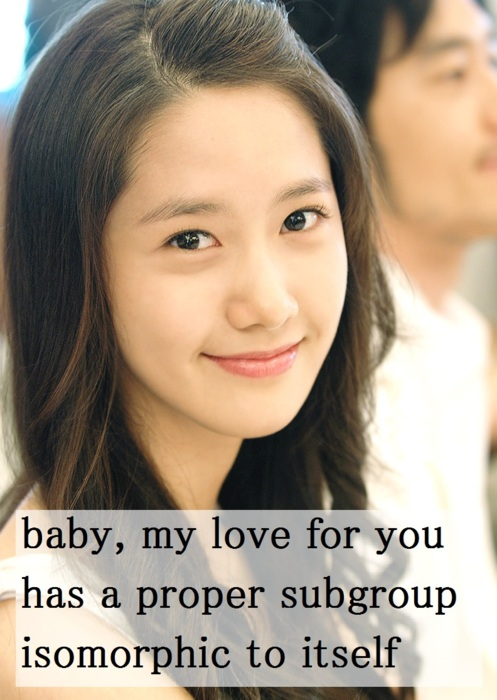
\includegraphics[height=8cm]{/home/evan/Pictures/TopologicalGG/love-proper-isomorphic-subgroup.jpg}
		%\caption{$\heartsuit$ is a group, $G \subsetneq \heartsuit$ a subgroup and $G \cong \heartsuit$.}
	\end{center}
	\begin{hint}
		Orders.
	\end{hint}
	\begin{sol}
		The point is that $\heartsuit$ is a group, $G \subsetneq \heartsuit$ a subgroup and $G \cong \heartsuit$.
		This can only occur if $\left\lvert \heartsuit \right\rvert = \infty$;
		otherwise, a proper subgroup would have strictly smaller size than the original.
	\end{sol}
\end{problem}

\begin{problem}
	Prove Lagrange's Theorem for Orders in the special case
	that $G$ is a finite abelian group.
	\begin{hint}
		Copy the proof of Fermat's Little Theorem, using
		\Cref{lem:group_mult_biject}.)
	\end{hint}
	\begin{sol}
		Let $\{g_1, g_2, \dots, g_n\}$ denote the elements of $G$.
		For any $g \in G$, this is the same as the set $\{gg_1, \dots, gg_n\}$.
		Taking the entire product and exploiting commutativity gives
		$g^n \cdot g_1g_2 \dots g_n = g_1g_2 \dots g_n$, hence $g^n=1$.
	\end{sol}
\end{problem}

\begin{problem}
	Show that $D_6 \cong S_3$.
	\begin{hint}
		Decide where the isomorphism should send $r$ and $s$,
		and the rest will follow through.
	\end{hint}
	\begin{sol}
		One can check manually that $D_6 \cong S_3$,
		using the map $r \mapsto (1 \; 2 \; 3)$ and $s \mapsto (1 \; 2)$.
	\end{sol}
\end{problem}

\begin{sproblem}
	Let $p$ be a prime.
	Show that the only group of order $p$ is $\ZZ_p$.
	\begin{hint}
		Generated groups.
	\end{hint}
	\begin{sol}
		Let $G$ be a group of order $p$, and $1 \neq g \in G$.
		Look at the group $H$ generated by $g$ and use Lagrange's Theorem.
	\end{sol}
\end{sproblem}

\begin{dproblem}
	[Cayley's Theorem]
	\gim
	Let $G$ be a finite group.\footnote{
		In other words, permutation groups can be arbitrarily weird.
		I remember being highly unsettled by this theorem when I first heard of it.}
	Show that there exists a positive integer $n$ such that
	\begin{enumerate}[(a)]
		\ii (Cayley's Theorem) $G$ is isomorphic to some subgroup of the symmetric group $S_n$.
		\ii (Representation Theory) $G$ is isomorphic to some subgroup of
		of the general linear group $\GL_n(\RR)$.
		(This is the group of invertible $n \times n$ matrices.)
	\end{enumerate}
	\label{thm:cayley_theorem}
	\begin{hint}
		Use $n = \left\lvert G \right\rvert$.
	\end{hint}
	\begin{sol}
		The idea is that each element $g \in G$ can be thought of as a permutation
		$G \to G$ by $x \mapsto gx$.
	\end{sol}
\end{dproblem}

\begin{problem}
	[MOP 2006] \gim
	There are $n$ markers, each with one side white and the other side black.
	In the beginning, these $n$ markers are aligned in a row so that their white sides are all up.
	In each step, if possible, we choose a marker whose white side is up (but not one of the outermost markers),
	remove it, and reverse the closest marker to the left of it and also reverse the closest marker to the right of it.
	
	Prove that if $n \equiv 1 \pmod 3$ it's impossible to reach a state with only two markers remaining.
	% http://www.artofproblemsolving.com/Forum/viewtopic.php?f=41&t=90046&p=3573800
	\begin{hint}
		Draw inspiration from $D_6$.
	\end{hint}
	\begin{sol}
		We have $www = bb$, $bww = wb$, $wwb = bw$, $bwb = ww$.
		Interpret these as elements of $D_6$.
	\end{sol}
\end{problem}


%\begin{problem}[Hard]
%	Exhibit two groups $G$ and $H$ which are not isomorphic with the property that
%	for every positive integer $n$,
%	the number of elements $g \in G$ with $\ord g = n$
%	equals the number of elements $h \in H$ with $\ord h = n$.
%\end{problem}
